\documentclass[conference]{IEEEtran}
\IEEEoverridecommandlockouts
\usepackage{amsmath,amssymb}
\usepackage{graphicx}
\usepackage{booktabs}
\usepackage{array}
\usepackage{algorithm}
\usepackage{algpseudocode}
\usepackage{cite}
\usepackage{url}
\usepackage{balance}
\usepackage{textcomp}
\newcommand{\TODO}[1]{\textbf{[TODO: #1]}}
\newcommand{\ours}{\textsc{Ours}}
\graphicspath{{figs/}}
\setlength{\textfloatsep}{7pt plus 2pt minus 2pt}
\setlength{\floatsep}{6pt plus 2pt minus 2pt}
\setlength{\intextsep}{6pt plus 2pt minus 2pt}
\setlength{\abovecaptionskip}{3pt}
\setlength{\belowcaptionskip}{0pt}
\def\BibTeX{{\rm B\kern-.05em{\sc i\kern-.025em b}\kern-.08em T\kern-.1667em\lower.7ex\hbox{E}\kern-.125em X}}

\begin{document}

\title{A Unified Task-Oriented Multimodal Semantic Communication Framework in 6G Networks: Deadline-Aware Camera--LiDAR Feature Sharing for Cooperative Perception}

\author{\IEEEauthorblockN{Hassan Ali}
\IEEEauthorblockA{\textit{Department of Artificial Intelligence}\\
\textit{FAST National University of Computer}\\
\textit{and Emerging Sciences (FAST-NUCES)}\\
Roll no.\ 24I-0047\\
i240047@isb.nu.edu.pk}
\and
\IEEEauthorblockN{Muhammad Saad}
\IEEEauthorblockA{\textit{Department of Artificial Intelligence}\\
\textit{FAST National University of Computer}\\
\textit{and Emerging Sciences (FAST-NUCES)}\\
Roll no.\ 24I-0058\\
i240058@isb.nu.edu.pk}}

\maketitle

\begin{abstract}
Vehicles can detect more objects when they share intermediate bird's-eye-view (BEV) features, but the shared bytes must cross a link with a rate limit and a deadline, and the sensors that produce them may be degraded. Many selection methods pick features by confidence and score accuracy once all messages have arrived. This paper studies a training-free policy that ranks BEV tiles by the sender's confidence and a sensor-quality proxy, the receiver's need, and a critical-region prior, and that sends only as many tiles as can still arrive before the deadline. Detection quality is scored as the average precision (AP) of whatever result is ready at the deadline, with an ego-only fallback. The policy is tested on a frozen HEAL detector, using the 16 OPV2V test scenes (2,170 frames), an emulated 5\,Mb/s link with 10\% loss, and degraded LiDAR and camera inputs. With two LiDAR cars and 10 link traces, the policy reaches AP@0.7 of 0.796 against 0.792 for a confidence-only selector (difference +0.40 points, 95\% interval [+0.23, +0.59]) and sends 35\% fewer bytes. When the receiving car has only a camera, the gain over the same selector is +2.42 points [+1.75, +3.33]. The sender-quality term accounts for most of the accuracy gain. The receiver-need term and deadline admission do not raise accuracy; admission saves bytes. Random and uniformly compressed sharing score below ego-only with a frozen fusion network. The link is emulated and the detector is not retrained, so the results are controlled measurements, not claims about deployed networks.
\end{abstract}

\begin{IEEEkeywords}
cooperative perception, task-oriented communication, deadline-aware transmission, BEV feature selection, V2V, 6G
\end{IEEEkeywords}

\section{Introduction}
A single vehicle cannot see around a truck or past the range of its LiDAR. Two vehicles that exchange intermediate BEV features can detect objects that neither sees alone \cite{xu2022opv2v,lu2024heal}. The network limits this exchange. Bytes are scarce, packets get lost, and a feature that arrives late is useless because the driving decision has already been made. The sensors add a second problem. Rain, glare, dropped LiDAR returns and short outages lower the quality of the features that are shared. Task-oriented (semantic) communication for vehicles \cite{feng2025,cao2025,sheng2026,liu2025,hu2026prag} addresses the first problem, and most of it reports accuracy after the messages have arrived. The work is motivated by the 6G (IMT-2030) vision \cite{itu2023}, but only an emulated link is used.

This work asks a narrow question: \emph{at a fixed byte budget and deadline, under sensor and link degradation at the same time, which BEV tiles should a car send, and should it send anything at all?} Existing selectors rank tiles by the sender's confidence \cite{hu2022where2comm}, by supply and demand \cite{xu2025cosdh}, or by uncertainty \cite{mukhopadhyay2026}. Some of them test latency or packet loss \cite{mukhopadhyay2026,wang2025jigsaw}. Among the studies reviewed (Section~\ref{sec:related}), none combines sender sensor quality, receiver need and a packet-level deadline in a common frozen detector, and none scores AP of the result available at the deadline. The studies reviewed are a small sample, so no priority is claimed.

\textbf{Contributions.}
\begin{itemize}
\item A lightweight, training-free tile-selection policy. It combines sender confidence, a hand-made sender-quality proxy, receiver need from one-frame-old feedback, and a critical-region prior, with deadline admission and an ego-only fallback.
\item An evaluation protocol: AP at the deadline, packet-level byte accounting that includes headers and feedback, common-random-number loss traces, a paired scene-level bootstrap with Holm correction, and a failure analysis that assigns each missed object to a cause.
\item A controlled study on the OPV2V test split with a frozen HEAL detector, covering two LiDAR cars, a LiDAR ego car with a camera collaborator, and a camera ego car with a LiDAR collaborator.
\item Negative results reported in full: two of three hypotheses are supported, one is not; random or uniform sharing is worse than no sharing; and a masking bug in the public HEAL code at non-square ranges, found and fixed during the work.
\end{itemize}
Section~\ref{sec:related} reviews related work, Section~\ref{sec:method} defines the method, Section~\ref{sec:setup} the experiments, Sections~\ref{sec:results}--\ref{sec:ablation} give results, comparison and ablations, and Sections~\ref{sec:discussion} and \ref{sec:conclusion} discuss limits and conclude.

\section{Related Work}\label{sec:related}
\textbf{Task-oriented communication for driving.} Semantic communication has been applied to edge-assisted driving \cite{feng2025}, stereo 3D detection \cite{cao2025}, lane-change planning \cite{zhang2026lane}, sensing--communication integration \cite{yang2025} and multimodal vehicle networks \cite{du2025}. Platform studies include near-sensor feature extraction for roadside perception \cite{zhang2025near} and V2V/V2I semantic-communication experiments \cite{li2025}. These works mostly report rate, latency or planning metrics; only \cite{cao2025} reports detection AP, with a single stereo camera.

\textbf{Communication-\allowbreak efficient cooperative perception.} Where2comm \cite{hu2022where2comm} shares features chosen from a spatial confidence map. CoSDH \cite{xu2025cosdh} combines the sender's confidence with the receiver's low point density. WhisperNet \cite{chen2026whisper} lets the receiver plan the budget. PragComm \cite{hu2026prag} also chooses representations and collaborators and compensates delayed messages. S2CP \cite{liu2025} and \cite{sheng2026} study noisy channels. Timing is treated by CooperTrim \cite{mukhopadhyay2026} (latency and loss by masking), by Zhu et al.\ \cite{zhu2026} (freshness scheduling), by Fresh2comm \cite{wu2025fresh} (power allocation against the largest delay) and by JigsawComm \cite{wang2025jigsaw} (delay and drop tests).

\textbf{Heterogeneous fusion.} HEAL \cite{lu2024heal} fuses features from different sensor types with a pyramid network trained on OPV2V \cite{xu2022opv2v}. Its camera encoder follows Lift-Splat-Shoot \cite{philion2020} and its LiDAR encoder is PointPillars \cite{lang2019}.

Table~\ref{tab:related} summarises what the closest selectors decide and test (the scheduling work \cite{zhu2026,wu2025fresh} is not a feature selector and is omitted). The gap examined here is the combination of sender sensor quality, receiver need and a hard deadline under simultaneous sensor and link degradation, scored at the deadline. ``Not stated'' means the text read does not say, not that the paper excludes it.

\begin{table*}[t]
\caption{Summary of the closest studies. ``Deadline'' means a hard time limit on result availability.}\label{tab:related}
\centering\scriptsize\setlength{\tabcolsep}{3pt}
\begin{tabular}{>{\raggedright\arraybackslash}p{2.55cm}>{\raggedright\arraybackslash}p{3.5cm}>{\raggedright\arraybackslash}p{3.35cm}>{\raggedright\arraybackslash}p{2.0cm}>{\raggedright\arraybackslash}p{1.5cm}>{\raggedright\arraybackslash}p{3.35cm}}
\toprule
Study & What decides what is sent & Delay / loss / deadline & Sensor degradation & Trained & Metric and time point\\\midrule
Where2comm \cite{hu2022where2comm} & Sender confidence map; request map & None (bandwidth only) & Pose noise & Yes & AP@0.5/0.7, after reception\\
CoSDH \cite{xu2025cosdh} & Supply (confidence) $\times$ demand (low point density) & Latency 100/200 ms; loss and deadline not stated & Not stated & Yes & AP@0.5/0.7\\
WhisperNet \cite{chen2026whisper} & Sender saliency, receiver-planned budget & Not stated & Localisation noise & Yes & AP@0.5/0.7\\
CooperTrim \cite{mukhopadhyay2026} & Receiver temporal uncertainty & Latency 0--200 ms, loss 0--10\% by masking; deadline not stated & Localisation error & Yes & AP/IoU, no time point\\
JigsawComm \cite{wang2025jigsaw} & Learned utility per byte & Delay 0--500 ms, drop 0--20\%; no deadline & Pose noise & Yes & mAP@0.5/0.7, data volume\\
PragComm \cite{hu2026prag} & Learned message, representation and collaborator selection & Delay 0--500 ms with compensation & Pose error & Yes & AP@0.5/0.7, bytes\\
\textbf{This study} & Sender quality $\times$ confidence $\times$ receiver need $\times$ critical region & Packet-level rate, queue, loss, hard deadline; all bytes counted & LiDAR thinning, outages, camera darkness and blur, jointly with a bad link & No (frozen) & AP@0.7 of the result ready at the deadline\\
\bottomrule
\end{tabular}
\end{table*}

\section{Problem Formulation and Method}\label{sec:method}
\subsection{Setting}
Fig.~\ref{fig:arch} gives an overview and Algorithm~\ref{alg:policy} summarises one frame. One ego car A and one collaborator B drive in the same scene. Both cars run a frozen encoder that maps their raw sensor data to a BEV feature map. B sends part of its map to A over a link with rate $R$, queueing delay $Q$ and packet-loss probability $\rho$. A fuses what arrives with its own map and runs the detection head. The result is due at a deadline $D$ after the frame is captured. The task is 3D vehicle detection, scored by AP.

The feature map has 64 channels on a $100\times176$ grid with 0.8 m cells, covering $x\in[-70.4,70.4]$ m and $y\in[-40,40]$ m. A \emph{tile} is $2\times2$ cells (1.6 m), which gives $N_T=4{,}400$ tiles of $4\times64=256$ values.

\subsection{Tokens and byte accounting}
A tile is quantised to $q=8$ bits per value and sent as a \emph{token}: 256 bytes plus 6 bytes of metadata (tile index, modality, scale, flags), 262 B in total. Four tokens share one packet, and each packet adds 72 B of application and link header. Sending $K$ tokens therefore costs
\begin{equation}
L(K)=262\,K+72\left\lceil K/4\right\rceil\ \text{bytes}.\label{eq:bytes}
\end{equation}
The receiver also sends a feedback message of 584 B per frame (a $32\times16$ confidence map at 8 bits plus headers). The per-frame budget $B$ covers both, so the largest affordable token count is $K_{\mathrm{cap}}=\max\{K: L(K)+584\le B\}$. For $B=16$ KiB (16,384 B) this is $K_{\mathrm{cap}}=56$ tokens (15,680 B plus 584 B). A lost packet still costs its bytes and time.

\subsection{Tile score}
Each tile $i$ of the collaborator's map receives
\begin{equation}
s_i=a_i\,r_i\,p_i\,(1+\lambda c_i)\,\bigl[\varepsilon+(1-\varepsilon)(1-e_i)\bigr]\,e^{-\mathrm{age}/\tau}.\label{eq:score}
\end{equation}
Here $a_i\in\{0,1\}$ says whether the sensor observed the tile (the Iverson bracket $[\,\cdot\,]$ below is 1 if the condition holds and 0 otherwise), $p_i\in[0,1]$ is the sender's own occupancy confidence, and $c_i\in\{0,1\}$ marks the \emph{critical region} (0--40 m ahead, $|y|<10$ m of the ego car). The term $e_i\in[0,1]$ is the receiver's confidence at that location, taken from the feedback message; a tile the receiver already sees well ($e_i\to1$) is down-weighted but never zeroed because $\varepsilon>0$. Feedback comes from the previous frame, is warped with the logged poses (never a future pose), and expires after 200 ms, after which $e_i=0$. The factor $\exp(-\mathrm{age}/\tau)$ lowers the score of old features; all tiles of one frame share one age, so it cannot change their ranking. The constants $\varepsilon=0.1$, $\lambda=1$ and $\tau=100$ ms were fixed in Phase 2, before any result existed, and were not tuned.

The sender-quality proxy $r_i\in[0,1]$ is hand-made, because the plan to train a quality head was dropped (Section~\ref{sec:deviations}). For a LiDAR sender, with $n_i$ points in the tile,
\begin{equation}
r_i=\min\!\bigl(1,\ \ln(1+n_i)/\ln(1+12)\bigr),\ \ a_i=[\,n_i>0\,].\label{eq:rlidar}
\end{equation}
For a camera sender, with mean brightness $\beta$ and Laplacian variance $\ell$ of the image region seen by the tile,
\begin{equation}
r_i=\min(1,\beta/0.40)\cdot\min\!\bigl(1,\sqrt{\ell/0.004}\bigr).\label{eq:rcam}
\end{equation}
The constants 12, 0.40 and 0.004 were also fixed before any result was seen.

\subsection{Deadline admission and output rule}
Before sending, the sender predicts when a cooperative result would be ready and admits only tokens that fit. With $t_{\mathrm{ready}}$ the time at which the sender's encoding and selection finish, $\hat R$ a causal estimate of the link rate (an exponential moving average, weight 0.2, started at 5 Mb/s) and $T_{\mathrm{res}}$ the receiver's 95th-percentile decode, fusion and detection time, the admitted count is
\begin{equation}
K^\ast=\max\Bigl\{K\le K_{\mathrm{cap}}:\ t_{\mathrm{ready}}+Q+\tfrac{8000\,L(K)}{\hat R}+T_{\mathrm{res}}\le D\Bigr\}.\label{eq:admit}
\end{equation}
The queue delay $Q$ is in ms, $\hat R$ in bit/s. If the ego encoder finishes later than the last packet, the receiver waits for it. Tokens that arrive intact before $D-T_{\mathrm{res}}$ are fused. At $D$ the system outputs the cooperative result if it is ready, otherwise the ego-only result if that is ready, otherwise an empty prediction:
\begin{equation}
y_D=\begin{cases}\text{cooperative} & t_{\mathrm{coop}}\le D\\ \text{ego-only} & t_{\mathrm{coop}}>D,\ t_{\mathrm{ego}}\le D\\ \text{empty} & \text{otherwise.}\end{cases}\label{eq:output}
\end{equation}
Objects stay in the AP denominator when the output is empty. Fig.~\ref{fig:timeline} shows the timeline for the main condition.

\begin{figure*}[t]
\centering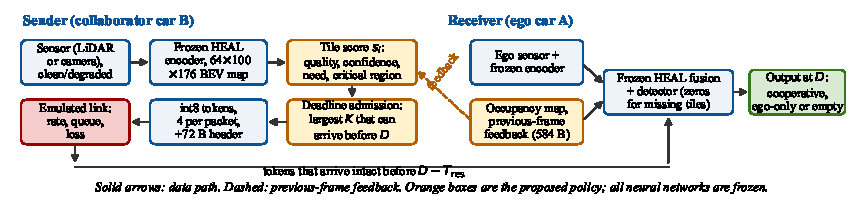
\includegraphics[width=0.95\textwidth]{fig1_architecture.pdf}
\caption{System overview. Orange boxes are the proposed policy; blue boxes are frozen HEAL components. The link is emulated. At the deadline the receiver outputs the best result that is ready.}\label{fig:arch}
\end{figure*}

\begin{algorithm}[t]
\caption{Per-frame selection and delivery}\label{alg:policy}
\begin{algorithmic}[1]
\Require collaborator map $F$, tile inputs $(a,r,p,c)$, feedback $e$ (previous frame), budget $B$, deadline $D$, rate estimate $\hat R$
\State $s_i\gets$ Eq.~\eqref{eq:score} for all tiles; rank tiles by $s_i$
\State $K_{\mathrm{cap}}\gets\max\{K: L(K)+584\le B\}$
\State $K^\ast\gets$ largest $K\le K_{\mathrm{cap}}$ satisfying Eq.~\eqref{eq:admit} (0 if none)
\State quantise the top $K^\ast$ tiles to int8 tokens; pack 4 per packet
\State send over the link; each packet is lost with probability $\rho$
\State \textbf{receiver:} zero-fill missing tiles; fuse tokens that arrived before $D-T_{\mathrm{res}}$ with the ego map; detect
\State update $\hat R$ from delivered packets
\State output $y_D$ by Eq.~\eqref{eq:output}
\end{algorithmic}
\end{algorithm}

\subsection{Objective and changes since Phase 2}
No network is trained, so there is no loss function. The design target is to maximise $\mathrm{AP}_D$, the AP of the outputs $y_D$ over the test frames, subject to at most $B$ bytes per frame. The instructor feedback after Phase 2 asked for a clearer novelty argument and a comparison with existing work (Section~\ref{sec:related}, Table~\ref{tab:related} and Section~\ref{sec:base}); the metric, conditions, baselines, hypotheses and decision rules were not changed. Implementation changes are listed in Section~\ref{sec:deviations}; the main one is that feedback is causal (previous frame), which the first run did not have.

\section{Experimental Setup}\label{sec:setup}
\subsection{Data, model and conditions}
\textbf{Data.} OPV2V \cite{xu2022opv2v}, official test split: 16 scenes, 2,170 frames. No validation split was downloaded and no training was done, so nothing was tuned on any data. For each scene one car pair (ego, collaborator) is fixed from logged poses alone, before any detection result: the two cars with the smallest mean distance. One scene has only two cars, more than 70 m apart in 119 of its 178 frames; those frames are ego-only for every method. Evaluation range is $x\in[-70.4,70.4]$ m, $y\in[-40,40]$ m.

\textbf{Model.} The official HEAL\_OPV2V checkpoint \cite{lu2024heal} (\texttt{heter\_pyramid\_collab}, PointPillars LiDAR encoder \cite{lang2019}, Lift-Splat-Shoot camera encoder \cite{philion2020}) is used as released. Encoders run once per frame and their 64-channel BEV features are cached; the fusion network and detection head are run for each method.

\textbf{Conditions.} C0: clean sensors and a good link (20 Mb/s, no loss, no queue). C1: degraded sensors, same link. C2: clean sensors and a bad link (5 Mb/s, 10\% loss, 20 ms queue). C3: degraded sensors and the bad link, the main condition. Degradation thins LiDAR to 50\% of its points and adds 3-frame outage bursts on 10\% of frames; for cameras it halves brightness and applies Gaussian blur ($\sigma=1.5$ px). The defaults are $D=100$ ms, $B=16$ KiB, 8-bit tokens and $\varepsilon,\lambda,\tau=0.1,1,100$ ms; they were set in Phase 2 and not tuned. A held-out stress condition keeps 30\% of LiDAR points and puts outages on 30\% of frames, at the same defaults.

\subsection{Experiments, baselines and ablations}
\textbf{Experiments.} Experiment A, the main one, uses two LiDAR cars, because it isolates the policy from modality effects. Experiment B uses a LiDAR ego car and a camera collaborator ($D=250$ ms). Experiment C uses a camera ego car and a LiDAR collaborator ($D=150$ ms). The primary deadline of 100 ms is infeasible when a camera is involved on this hardware (Section~\ref{sec:timing}).

\textbf{Baselines.} B0: ego only, no communication. B1: uniform compression of the whole BEV map (block-averaged tokens at the finest resolution that fits the budget). B2: random tiles. B3: confidence-only, which ranks tiles by the sender's occupancy confidence $p_i$ (a Where2comm-style selector inside the same frozen detector). U0: all tiles over an instant link, a reference and not an upper bound. All methods use the same frames, car pairs, link draws, byte cap and deadline. A fifth baseline, PragComm \cite{hu2026prag}, was cut for time.

\textbf{Ablations.} A1: no quality term ($r_i=1$). A2: no receiver-need term. A3: no deadline admission (send $K_{\mathrm{cap}}$ tokens). A7: oracle same-frame feedback. R1: one retransmission of lost packets, paying the same bytes and time.

\subsection{Metrics and statistics}
The main metric is AP at IoU 0.7 (AP@0.7) of the result available at the deadline; AP@0.5 is also reported. \emph{Critical recall} is recall inside the critical region at IoU 0.5. Bytes per frame include headers and feedback. Precision, recall and F1 are computed at a fixed score threshold of 0.5, chosen in advance. Plain accuracy (correct over total) is not defined for detection, because empty space has no count of correct rejections, so AP is used.

Differences are paired bootstrap over scenes (2,000 resamples of the 16 scenes, seed 0) with Holm adjustment over the family of tests. A frame-block bootstrap (blocks of 20 frames) is also computed and is labelled as such in the logs. Loss draws are common random numbers: a SHA-256 hash of (scene, frame, trace, packet index) gives each packet the same uniform draw for every method. The main runs use 3 link traces (indices 0--2); the pre-declared H1 test uses 10 (0--9). Outage schedules use a fixed seed (11).

\textbf{Hypotheses.} H1: in C3, ours has higher AP@0.7 than B3. H2: deadline admission raises critical-region recall. H3: in C0, ours is non-inferior to B3 (margin $-1$ point), and in C3 ours sends at least 25\% fewer bytes at matched AP.

\subsection{Implementation and hardware}\label{sec:timing}
All timing is emulated. Stage latencies were measured on one RTX 5050 Laptop GPU (8 GB, fp32) in WSL2 Ubuntu with 7.7 GB of RAM and replayed in a discrete-event timeline. For the LiDAR pair: encoder 9.7 ms, selection and quantisation 2.0 ms, $T_{\mathrm{res}}=50.4$ ms and ego-only detection 42.7 ms (95th percentile), so an ego-only result is ready at about 52 ms. A camera encoder took 223 ms at first; profiling showed 179 ms in the voxel-pooling step, and an equivalent scatter-add re-implementation brought it to 68.7 ms (relative difference 4e-4 to the original). Even so, a camera collaborator cannot deliver a cooperative result before about 165 ms.

Software: Python 3.10, PyTorch 2.11 (CUDA 12.8, required by the RTX 5050) and NumPy 1.26. The public HEAL code needed small patches to run on this GPU (for example a replacement for \texttt{spconv}); model logic, loss and evaluation code were not changed, with one exception. HEAL's fusion code masks camera agents with a crop start index $H/2-\text{crop}_H/2$, which is $-12$ at this non-square range. Python slicing reads it as ``12 from the end'', which leaves only 12 of 100 rows (8\%) of the camera map unmasked. The indices were clamped; LiDAR-only runs are unaffected. A first camera diagnostic made before the fix wrongly concluded that frozen HEAL ignores camera collaborators; all camera runs were repeated after the fix and the earlier ones discarded. As a fidelity check, stock HEAL inference on the chosen car pairs at the evaluation range gives AP@0.3/0.5/0.7 of 0.98/0.97/0.94, in line with the unconstrained reference U0 in C0 (Table~\ref{tab:main}). The official all-car HEAL run could not be reproduced because \texttt{spconv} is unavailable on this GPU. Code: see the repository in the Declarations.

\subsection{Deviations from the original plan}\label{sec:deviations}
Table~\ref{tab:dev} lists every difference between the Phase 2 methodology and what was run, with the reason.

\begin{table*}[t]
\caption{Deviations from the Phase 2 plan (from the project changes log).}\label{tab:dev}
\centering\scriptsize\setlength{\tabcolsep}{3pt}
\begin{tabular}{r >{\raggedright\arraybackslash}p{4.6cm} >{\raggedright\arraybackslash}p{5.2cm} >{\raggedright\arraybackslash}p{6.2cm}}
\toprule
\# & Phase 2 plan & What was done & Reason and effect\\\midrule
1 & Train encoders, adapters, quality and fusion heads & No training; frozen official HEAL checkpoint & Limited time and an 8 GB laptop GPU\\
2 & Learned quality head & Hand-made proxies (Eqs.~\ref{eq:rlidar}, \ref{eq:rcam}), constants fixed beforehand & No training; called ``proxy''\\
3 & Learned masked fusion head & HEAL's pretrained fusion; missing tiles are zeros & Fusion not tuned to dropped tiles; may hurt all methods\\
4 & Train / validation / test & Official test split only; defaults only & Validation split not downloaded; sweeps never used to pick values\\
5 & Camera and LiDAR on each car & One sensor per car (HEAL design) & Pretrained checkpoint design\\
6 & Official sensor assignment & Own pair assignment; other cars excluded & Official file has LiDAR+camera pairs in 7 of 16 scenes; mild distribution shift\\
7 & Nearest car as collaborator per frame & One fixed pair per scene, from poses only, before any result & Loader fixes the car list; one scene is ego-only in 119 of 178 frames\\
8 & Seeds are training seeds & Seeds change only loss draws and outages & No training\\
9 & B1 uniform compression, B4 PragComm & B1 added later; B4 cut & Time; no PragComm comparison\\
10 & Ablations A4, A5, A6 & Not applicable & A4 cannot change ranking (equal ages); A5 needs two sensors per car; A6 needs training\\
11 & Latency from a full pipeline on a lab GPU & Measured on the RTX 5050 laptop and replayed & Emulated system\\
12 & $T_{\mathrm{res}}$ from a validation split & 95th percentile on cached development frames & No validation split\\
13 & Depth supervision in the camera encoder & Disabled & Training loss only; no inference effect\\
14 & Original voxel pooling & Equivalent scatter-add & Original took 179 ms; features differ by 4e-4 (relative)\\
15 & Feature shape assumed 88$\times$50 tiles & Confirmed on real tensors: 4,400 tiles & None\\
16 & Detection range as in Phase 2 & $x\pm70.4$ m, $y\pm40$ m & Official HEAL numbers use $\pm102.4$ m; not directly comparable\\
17 & Primary deadline $D=100$ ms for all experiments & $D=100$ ms for Experiment A; 250 ms (B) and 150 ms (C) & Camera encoders are slow on this GPU (68.7 ms collaborator, 65.1 ms ego), so no cooperative result can be ready by 100 ms; AP is not comparable across experiments\\
\bottomrule
\end{tabular}
\end{table*}

\section{Results and Analysis}\label{sec:results}
\subsection{Two LiDAR cars (main experiment)}
Table~\ref{tab:main} and Fig.~\ref{fig:main} give the main comparison at $D=100$ ms and 16 KiB. Cooperation helps a great deal: in C0 the unconstrained reference U0 beats ego-only by +15.34 points (95\% CI [+12.39, +18.46]), and in C3 ours beats ego-only by +12.11 [+10.05, +14.34]. How tiles are chosen matters. Random sharing (B2, 0.669) and uniform compression (B1, 0.640) fall below ego-only (B0, 0.675) in C3, because the frozen fusion network was never trained on sparse or block-averaged features. Both confidence-based selectors recover most of the gap (3-trace means: B3 0.793, ours 0.796, U0 0.867).

\begin{table}[t]\caption{Main comparison, LiDAR ego car and LiDAR collaborator, condition C3 (degraded sensors and bad link), $D$ = 100 ms, 16 KiB budget. AP is the mean over 3 link traces. Critical recall is recall inside the critical region at IoU 0.5.}\label{tab:main}
\centering\scriptsize\setlength{\tabcolsep}{2.6pt}\begin{tabular}{lccccc}\toprule
Method & AP@0.5 & AP@0.7 & Crit.\ rec. & Bytes & C0 AP@0.7\\\midrule
Ego only & 0.785 & 0.675 & 0.730 & 0 & 0.783\\
Uniform & 0.752 & 0.640 & 0.722 & 11,278 & 0.752\\
Random & 0.760 & 0.669 & 0.743 & 14,506 & 0.798\\
Confidence-only & 0.878 & 0.793 & 0.928 & 14,506 & 0.910\\
\textbf{Ours} & \textbf{0.880} & \textbf{0.796} & \textbf{0.937} & \textbf{9,415} & \textbf{0.911}\\
Unconstrained & 0.933 & 0.867 & 0.968 & -- & 0.936\\
\bottomrule\end{tabular}\end{table}


\begin{figure*}[t]
\centering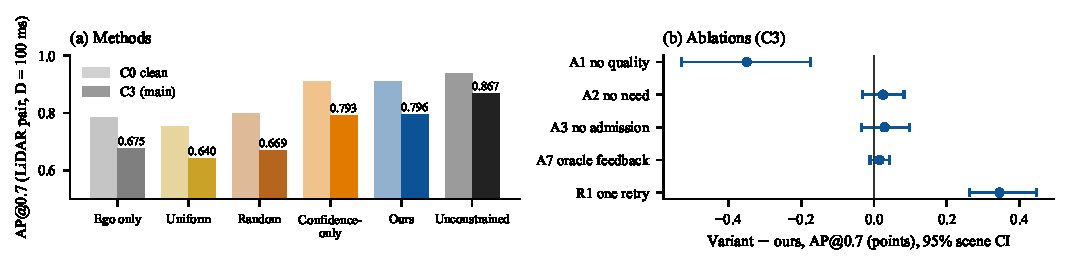
\includegraphics[width=\textwidth]{fig2_main_ablation.pdf}
\caption{(a) AP@0.7 for the LiDAR pair, clean (light) and degraded with a bad link (dark, labelled). Random and uniform sharing fall below ego-only. (b) Ablations: variant minus full policy with 95\% scene intervals; only removing the quality term and adding one retry move AP.}\label{fig:main}
\end{figure*}

\subsection{Statistical tests and hypotheses}
Table~\ref{tab:tests} lists the paired tests. \textbf{H1 is supported, with a small effect.} Over 10 link traces (B3 0.792, ours 0.796), ours exceeds B3 by +0.40 points [+0.23, +0.59]. The 3-trace run of Table~\ref{tab:main} (B3 0.793, ours 0.796) gives +0.36 [+0.20, +0.53]. At AP@0.5 the difference is +0.15 [+0.01, +0.28], which is not significant after Holm adjustment.

\textbf{H2 is not supported.} Critical-region recall in C3 is 0.937 with admission and 0.938 without, and removing admission changes AP@0.7 by $+0.03$ points [$-0.04$, $+0.10$] (Table~\ref{tab:abl}). Admission saves bytes; it does not raise recall.

\textbf{H3 is supported for non-inferiority and partly for bytes.} In C0, ours minus B3 is +0.05 points [$-0.08$, $+0.17$], inside the margin. In C3 ours sends 9,415 B per frame against 14,506 B for B3, 35\% fewer ($(14{,}506-9{,}415)/14{,}506$), with equal or higher AP. On a clean link admission never binds and the two selectors send nearly the same bytes (15,372 and 15,383 B), so the 25\% target is met only when the link is poor.

\begin{table}[t]\caption{Paired scene-level bootstrap (2,000 resamples over 16 scenes, Holm-adjusted $p$). $\Delta$ is the difference in AP@0.7 in percentage points. The first row uses 10 link traces, the others 3.}\label{tab:tests}
\centering\scriptsize\setlength{\tabcolsep}{2.5pt}\begin{tabular}{lccc}\toprule Comparison & $\Delta$ (pts) & 95\% CI & Holm $p$\\\midrule
H1: ours $-$ B3, C3 (10 traces) & +0.40 & [+0.23, +0.59] & $<$0.001\\
ours $-$ B3, C3 (3 traces) & +0.36 & [+0.20, +0.53] & 0.001\\
same, AP@0.5 & +0.15 & [+0.01, +0.28] & 0.175\\
ours $-$ B0, C3 & +12.11 & [+10.05, +14.34] & 0.001\\
ours $-$ B2, C3 & +12.69 & [+10.86, +14.79] & 0.001\\
ours $-$ B1, C3 & +15.61 & [+13.01, +18.37] & 0.001\\
H3: ours $-$ B3, C0 & +0.05 & [$-$0.08, +0.17] & 1.000\\
U0 $-$ B0, C0 & +15.34 & [+12.39, +18.46] & 0.001\\
\bottomrule\end{tabular}\end{table}


\subsection{Deadline, budget and link sweeps}
These are sweeps around the C3 operating point, not tuning (Fig.~\ref{fig:sweeps}). At $D=50$ ms even the ego-only result is late (about 52 ms), so every method outputs nothing and scores 0.000. At 75 ms no cooperative result can be ready, and all methods fall back to ego-only (0.675); ours sends 520 B per frame where B3 sends 14,506 B and wastes the link.

AP saturates by 16 KiB for the frozen detector: ours scores 0.783 at 8 KiB and 0.796 at 16 and 32 KiB, while B3 sends 28,948 B at a 32 KiB budget and ours 9,415 B. Fig.~\ref{fig:timeline} shows why admission binds: all 56 tokens would finish at 107.2 ms, 7 ms after the deadline, and 39 tokens fit at the nominal link rate (derived from the logged latencies and Eq.~\eqref{eq:bytes}).

\begin{figure*}[t]
\centering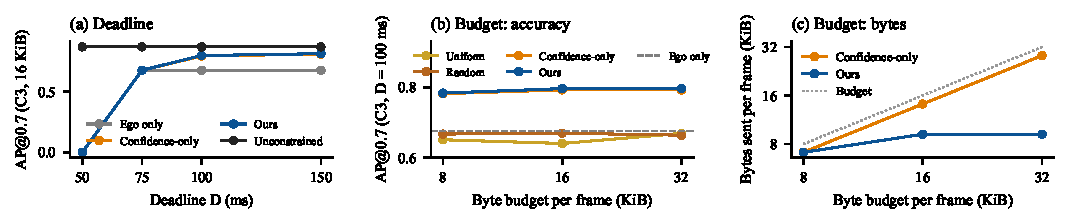
\includegraphics[width=\textwidth]{fig3_sweeps.pdf}
\caption{Sweeps around C3 for the LiDAR pair. (a) AP versus deadline: at 50 ms nothing is ready, at 75 ms all methods fall back to ego-only. (b) AP versus byte budget. (c) Bytes sent versus budget: confidence-only fills the budget, ours stops at what can arrive in time.}\label{fig:sweeps}
\end{figure*}

\begin{figure}[t]
\centering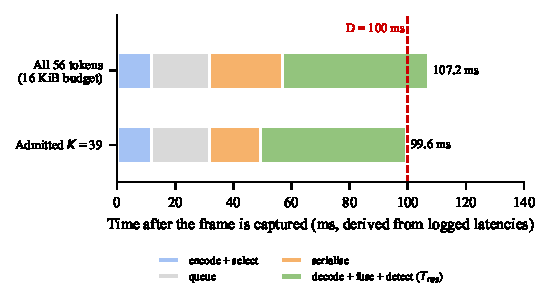
\includegraphics[width=\columnwidth]{fig5_timeline.pdf}
\caption{Timeline for the LiDAR pair in C3 (5 Mb/s, 20 ms queue). Sending all 56 tokens misses the deadline; admission sends fewer tokens. Values are derived from the logged latencies, not measured per frame.}\label{fig:timeline}
\end{figure}

Admission matters most on a very slow link: at 1 Mb/s ours scores 0.709 against 0.688 and sends 2,889 B against 14,566 B (80\% fewer). With a 40 ms queue nothing can arrive in time, so ours sends 523 B and B3 wastes 14,566 B. At 10 and 20 Mb/s ours and B3 differ by only 0.003.

\subsection{Camera experiments}
Table~\ref{tab:camera} and Fig.~\ref{fig:cam}(a),(b) give the two camera experiments. In Experiment B (LiDAR ego, camera collaborator), a clean camera adds +6.68 points over ego-only (U0 minus B0 in C0, [+4.99, +8.60]), but a degraded camera adds nothing: ours minus ego-only is $-0.22$ [$-1.02$, $+0.60$] in C3, and confidence-only sharing is slightly below ego-only ($-0.56$ [$-1.27$, $+0.13$], interval includes zero). Ours beats B3 by +0.34 [+0.09, +0.66] because the camera-quality proxy avoids bad tiles, but it does not turn a bad camera into a useful one.

In Experiment C (camera ego, LiDAR collaborator) the ego car is very weak alone: AP@0.7 is 0.164 clean and 0.000 degraded. LiDAR tiles lift this to 0.560 and 0.332. Ours minus B3 is +2.42 points [+1.75, +3.33] in C3, larger than in the LiDAR pair. Removing the quality term costs 1.51 points [+1.10, +1.90]. Admission has no effect on accuracy. A gap to U0 remains (0.332 against 0.550) because 16 KiB carries only 56 tokens; AP keeps rising with budget (Fig.~\ref{fig:cam}(b)) and the gain over B3 is +1.59 [+1.06, +2.21] at 8 KiB. It is +1.98 [+1.47, +2.65] at 32 KiB and +1.56 [+1.06, +2.14] at 64 KiB.

\begin{table}[t]\caption{AP@0.7 with one camera car. Experiment B: LiDAR ego, camera collaborator ($D$ = 250 ms). Experiment C: camera ego, LiDAR collaborator ($D$ = 150 ms). 16 KiB budget, 3 traces.}\label{tab:camera}
\centering\scriptsize\setlength{\tabcolsep}{4pt}\begin{tabular}{lcccc}\toprule & \multicolumn{2}{c}{Exp.\ B (LiDAR ego)} & \multicolumn{2}{c}{Exp.\ C (camera ego)}\\\cmidrule(lr){2-3}\cmidrule(lr){4-5}
Method & C0 & C3 & C0 & C3\\\midrule
Ego only & 0.783 & 0.674 & 0.164 & 0.000\\
Uniform & 0.424 & 0.391 & 0.117 & 0.000\\
Random & 0.789 & 0.666 & 0.175 & 0.003\\
Confidence-only & 0.858 & 0.668 & 0.553 & 0.307\\
\textbf{Ours} & \textbf{0.858} & \textbf{0.672} & \textbf{0.560} & \textbf{0.332}\\
Unconstrained & 0.850 & 0.675 & 0.710 & 0.550\\
\bottomrule\end{tabular}\end{table}


\begin{figure*}[t]
\centering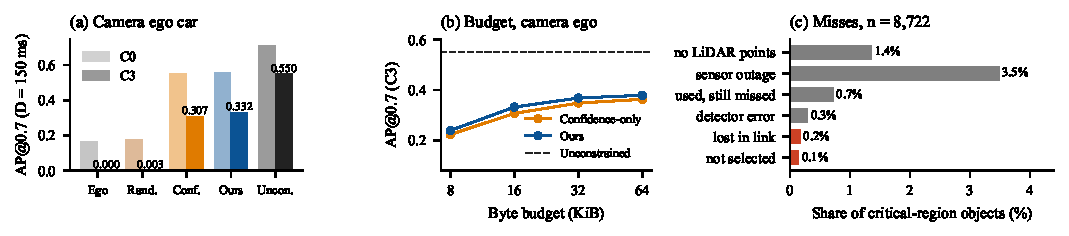
\includegraphics[width=\textwidth]{fig4_camera_failure.pdf}
\caption{(a) Camera ego car with a LiDAR collaborator, $D=150$ ms: AP@0.7 clean (light) and degraded (dark, labelled). (b) AP versus byte budget for the camera ego car. (c) Causes of missed critical-region objects in C3 for the LiDAR pair; red bars are communication causes.}\label{fig:cam}
\end{figure*}

\subsection{Precision, recall and stress test}
Table~\ref{tab:pr} gives precision and recall. Precision is high for every method, about 0.98 at IoU 0.5 and 0.94 at IoU 0.7, so the frozen detector rarely reports objects that are not there. Cooperation changes recall: at IoU 0.5 it rises from 0.645 (ego only) to 0.704 (ours), while U0 reaches 0.783. Ours and B3 have the same precision and ours has slightly higher recall (0.704 against 0.699), in line with their small AP gap.

\begin{table}[t]\caption{Precision (P), recall (R) and F1 in C3 at a fixed score threshold of 0.5, chosen before the runs. Pooled over all frames and 3 link traces (83,148 ground-truth vehicles). No intervals are computed.}\label{tab:pr}
\centering\scriptsize\setlength{\tabcolsep}{3pt}\begin{tabular}{lcccccc}\toprule & \multicolumn{3}{c}{IoU 0.5} & \multicolumn{3}{c}{IoU 0.7}\\\cmidrule(lr){2-4}\cmidrule(lr){5-7}
Method & P & R & F1 & P & R & F1\\\midrule
Ego only & 0.984 & 0.645 & 0.779 & 0.914 & 0.599 & 0.724\\
Uniform & 0.989 & 0.525 & 0.686 & 0.928 & 0.493 & 0.644\\
Random & 0.992 & 0.561 & 0.717 & 0.944 & 0.533 & 0.682\\
Confidence-only & 0.985 & 0.699 & 0.817 & 0.943 & 0.669 & 0.783\\
\textbf{Ours} & 0.984 & 0.704 & 0.821 & 0.944 & 0.675 & 0.787\\
Unconstrained & 0.982 & 0.783 & 0.871 & 0.951 & 0.758 & 0.844\\
\bottomrule\end{tabular}\end{table}


In the stress condition (30\% of LiDAR points, 30\% outage frames) the ranking is unchanged: AP@0.7 is 0.505 for ego only, 0.628 for B3 and 0.635 for ours on the bad link. Ours minus B3 is +0.73 points [+0.49, +1.01] on the bad link and +0.71 [+0.47, +0.99] on the good link, larger than in C3 (+0.40), consistent with quality estimates mattering more when sensors are worse.

\subsection{Failure analysis}
For the LiDAR pair in C3 at IoU 0.5 (one link trace), 8,722 critical-region objects are present and ours detects 8,182 (93.8\%). Of the rest, 3.5\% fall on sensor-outage frames, 1.4\% have no LiDAR points, 0.7\% were used but still missed, 0.3\% are missed even with all features (U0 misses them too), 0.2\% are lost in transmission and 0.1\% were not selected. Communication choices (lost or not selected) account for 0.3\% of the objects; the rest are sensing limits (Fig.~\ref{fig:cam}(c)). At this budget the selector is not the bottleneck, so differences between selectors are small.

\section{Comparison with Base Papers}\label{sec:base}
\textbf{Summary of base papers.} Table~\ref{tab:base} lists the base studies on which the problem, method or setup rest. Reported results (asterisk) are quoted from each paper's abstract or our Phase 2 reading and are not comparable to this study's numbers.

\begin{table*}[t]
\caption{Base papers: problem, method, data, metric, reported result and limitation relative to this study. Starred results are quoted from the authors, not reproduced.}\label{tab:base}
\centering\scriptsize\setlength{\tabcolsep}{3pt}
\begin{tabular}{>{\raggedright\arraybackslash}p{1.9cm}>{\raggedright\arraybackslash}p{3.0cm}>{\raggedright\arraybackslash}p{3.1cm}>{\raggedright\arraybackslash}p{1.9cm}>{\raggedright\arraybackslash}p{3.0cm}>{\raggedright\arraybackslash}p{3.7cm}}
\toprule
Paper & Problem & Method & Data & Reported result$^*$ & Limitation for this gap\\\midrule
Where2comm \cite{hu2022where2comm} & Bandwidth-limited cooperative detection & Confidence map selects what to send & OPV2V and 3 others & More than 100,000$\times$ lower communication volume on OPV2V, still ahead of DiscoNet and V2X-ViT & No delay or loss model; no sensor degradation; trained\\
CoSDH \cite{xu2025cosdh} & Accuracy versus bandwidth & Supply--demand selection, intermediate--late hybrid & Simulated and real & State-of-the-art accuracy and bandwidth trade-off (no single number in the abstract) & Loss, queue and deadline not stated; trained\\
PragComm \cite{hu2026prag} & Pragmatic message design & Selects message, representation and collaborators; delay compensation & OPV2V & Matching prior detection with more than 32.7K-fold less volume & Heterogeneity and delay studied; does not isolate joint modality failure and a hard deadline\\
S2CP \cite{liu2025} & Noisy, constrained networks & Dilated cross-attention, codec, MAE pre-training & V2XSet, V2V4Real & +10.80\% AP and 75\% less volume against Select2Col on V2XSet with AWGN & LiDAR only; no joint camera--LiDAR failure; no deadline\\
\bottomrule
\end{tabular}
\end{table*}

\textbf{Quantitative comparison.} A side-by-side table of AP values against these papers would be misleading. They train their own models, use different agent counts, ranges and bandwidth definitions, and score AP after all messages arrive. This study instead re-implements the core idea of the closest selector inside its own protocol: B3 is a Where2comm-style confidence selector in the same frozen detector, on identical frames, link draws and bytes. All results against B3 are therefore re-implemented, not quoted. The base methods CoSDH, WhisperNet, CooperTrim and PragComm were not re-implemented.

\textbf{Methodological difference.} The base papers train a selector or fusion network to cope with missing tiles. This study keeps the detector frozen and changes only the policy: a sender-quality term, a receiver-need term, a critical-region prior and a packet-level deadline rule, scored on the result available at the deadline. These additions target the observation that the base papers do not test sensor and link degradation together.

\textbf{Improvement analysis.} Against B3 in C3 (LiDAR pair, 10 traces) ours gains +0.40 points absolute (0.792 to 0.796, about 0.5\% relative) with 35\% fewer bytes. For the camera ego car the gain is +2.42 points (0.332 against 0.307, about 8\% relative). The gain comes from the sender-quality term (+0.35 points in the LiDAR pair, +1.51 in Experiment C, Section~\ref{sec:ablation}); the need term and admission add nothing to accuracy.

\textbf{Fairness and limits.} The comparison with B3 is fair in data, bytes, link and detector, but B3 is one reading of confidence-only selection, not the published, trained Where2comm. This study does not outperform trained methods on their own settings and does not claim to. On clean data ours is only non-inferior to B3, not better.

\section{Ablation Study}\label{sec:ablation}
Table~\ref{tab:abl} and Fig.~\ref{fig:main}(b) show the C3 ablations. Removing the quality term (A1) costs 0.35 points [0.18, 0.53] in Experiment A and 1.51 in Experiment C: it is the component that helps. Removing the receiver-need term (A2) changes AP by +0.02 points with an interval that includes zero; in Experiment C it raises AP slightly (+0.25 points [+0.10, +0.39]). The need term makes the policy send more bytes (9,415 against 8,894) for no accuracy benefit. A possible, untested reason is that the feedback map comes from the ego car's own detector, a poor guide to what a weak ego car lacks. Removing admission (A3) changes AP by +0.03 points with an interval that includes zero, but sends 54\% more bytes (14,495 against 9,415). Oracle same-frame feedback (A7) adds +0.02 points, so causal feedback costs nothing measurable. One retransmission (R1) is worth +0.35 points for about 265 B per frame. A4--A6 are not applicable (Table~\ref{tab:dev}).

\begin{table}[t]\caption{Ablations in C3 (the full policy has AP@0.7 = 0.796 in Experiment A). Variant $-$ ours, in AP@0.7 points with 95\% scene CI, for Experiment A (LiDAR pair) and Experiment C (camera ego).}\label{tab:abl}
\centering\scriptsize\setlength{\tabcolsep}{4pt}\begin{tabular}{lcc}\toprule Variant & $\Delta$ Exp.\ A & $\Delta$ Exp.\ C\\\midrule
Ours (full) & -- & --\\
A1 no quality & $-$0.35 [$-$0.53, $-$0.18] & $-$1.51 [$-$1.90, $-$1.10]\\
A2 no need & +0.02 [$-$0.03, +0.08] & +0.25 [+0.10, +0.39]\\
A3 no admission & +0.03 [$-$0.04, +0.10] & 0.00 [0.00, 0.00]\\
A7 oracle feedback & +0.02 [$-$0.01, +0.04] & --\\
R1 one retry & +0.35 [+0.26, +0.45] & --\\
\bottomrule\end{tabular}\end{table}


\section{Discussion and Limitations}\label{sec:discussion}
\textbf{Why it works, and where it does not.} The gain comes from not sending tiles the sender cannot trust: few LiDAR points, or a dark, blurred image. Confidence-only ranking ignores how well a tile was observed. The effect is small when the receiver is strong and the budget already carries the best tiles (+0.40 points), and larger when the receiver is weak (+2.42) or sensing is worse (stress, +0.73). Admission mainly avoids wasting traffic. The study shows no effect on driving safety; AP and recall are proxies. Random and uniform sharing hurt because the frozen fusion network was not trained on sparse or compressed features, so a good selector is a precondition.

\textbf{Were the Phase 1 and 2 objectives met?} Partly. H1 and H3 hold and H2 does not. The practical target of 3 points over a confidence-only selector was not reached in Experiment A (+0.40) or C (+2.42). The target of at least 25\% fewer bytes at matched accuracy was met on the lossy link only.

\textbf{Limitations and threats to validity.} (i) \emph{Scale:} 16 test scenes, one of them mostly ego-only. Intervals for the LiDAR pair are narrow but the effects are small, and some intervals (for example ours minus ego-only in Experiment B) include zero; results may not transfer to other scenes. (ii) \emph{No training or validation split:} the results describe a policy on a pretrained model, with nothing tuned. (iii) \emph{Emulated link and timing:} a simulated link with independent loss and latencies from one laptop GPU; no real 6G or radio behaviour is measured. (iv) \emph{Proxies:} the quality estimates are hand-made, and confidence and need come from the model's own occupancy output. (v) \emph{Setup:} one car pair per scene, one sensor per car, a range of $\pm70.4\times\pm40$ m instead of $\pm102.4$ m, and a mild distribution shift from the sensor assignment (Table~\ref{tab:dev}). (vi) \emph{Missing pieces:} no PragComm baseline, no real-data transfer (for example V2V4Real \cite{xu2023v2v4real}), no pose noise, and no qualitative BEV visualisation of the selected tiles.

\section{Conclusion and Future Work}\label{sec:conclusion}
A training-free policy that ranks BEV tiles by sender quality and confidence, adds a receiver-need term and a critical-region prior, and admits only tiles that can arrive before the deadline gave a small, statistically reliable accuracy gain over a confidence-only selector (+0.40 points AP@0.7, 10 link traces) with 35\% fewer bytes on a lossy link, and a larger gain (+2.42 points) for a camera-only ego car. The sender-quality term is the useful part; the need term and admission did not raise accuracy. Future work: train a fusion head on masked tiles, add PragComm and a real dataset such as V2V4Real, learn the quality proxy, test more car pairs, and use a validation split to set the policy constants.

\section*{Declarations}
\textbf{Data and code availability.} OPV2V \cite{xu2022opv2v} and the HEAL checkpoint \cite{lu2024heal} are public. The code, logs and figures behind every number are in the public repository \url{https://github.com/Hassan07Ali/deadline-aware-semantic-comm-cooperative-perception}.

\textbf{Conflict of interest and funding.} The authors declare no conflict of interest and received no external funding.

\textbf{AI-tool usage.} The authors used Claude (Anthropic), through Claude Code, to help write and debug the experiment code, to make figures and tables from the saved logs, to look up and check references, and to draft and edit this text. The authors reviewed the content and take responsibility for it.

\textbf{Acknowledgements.} The authors thank Ms.\ Laraib Afzal for feedback.

\balance
\footnotesize
\bibliographystyle{IEEEtran}
\bibliography{refs}

\end{document}
